\section{Baterías de ion de litio (Li-ion)}

Las baterías de ion de litio se utilizan ampliamente en sistemas portátiles,
 como vehículos eléctricos y computadoras portátiles. Su uso extendido se 
 debe principalmente a su alta densidad energética, que oscila entre 100 y 265 Wh/Kg,
  o expresado en términos de densidad volumétrica, entre 250 y 670 Wh/L según se indica en 
  \cite{noauthor_lithium-ion_nodate}. Estas baterías tienen un rango de voltaje típico de
   3 a 4.2 voltios, lo que implica que se requiere una menor cantidad de celdas para
alcanzar voltajes elevados. Una celda presenta una larga vida, llegando a tener el 80\%
de su capacidad luego de 500 ciclos de carga \cite{texas_instrumens_multi-chemistry_2022}.


Las baterías Li-Ion presentan algunas desventajas, como su alta sensibilidad a la sobrecarga,
sobredescarga, corrientes altas, sobrecalentamiento, entre otros factores. Debido a estas características,
es necesario utilizar un circuito de protección, como un BMS (\textit{Battery Management System}), para garantizar
su funcionamiento seguro y prolongar su vida útil \cite{texas_instrumens_multi-chemistry_2022}. En la figura 
\ref{fig:liion} se pueden observar baterías de iones de litio en diferentes formatos.

\begin{figure}[H]
   \centering
   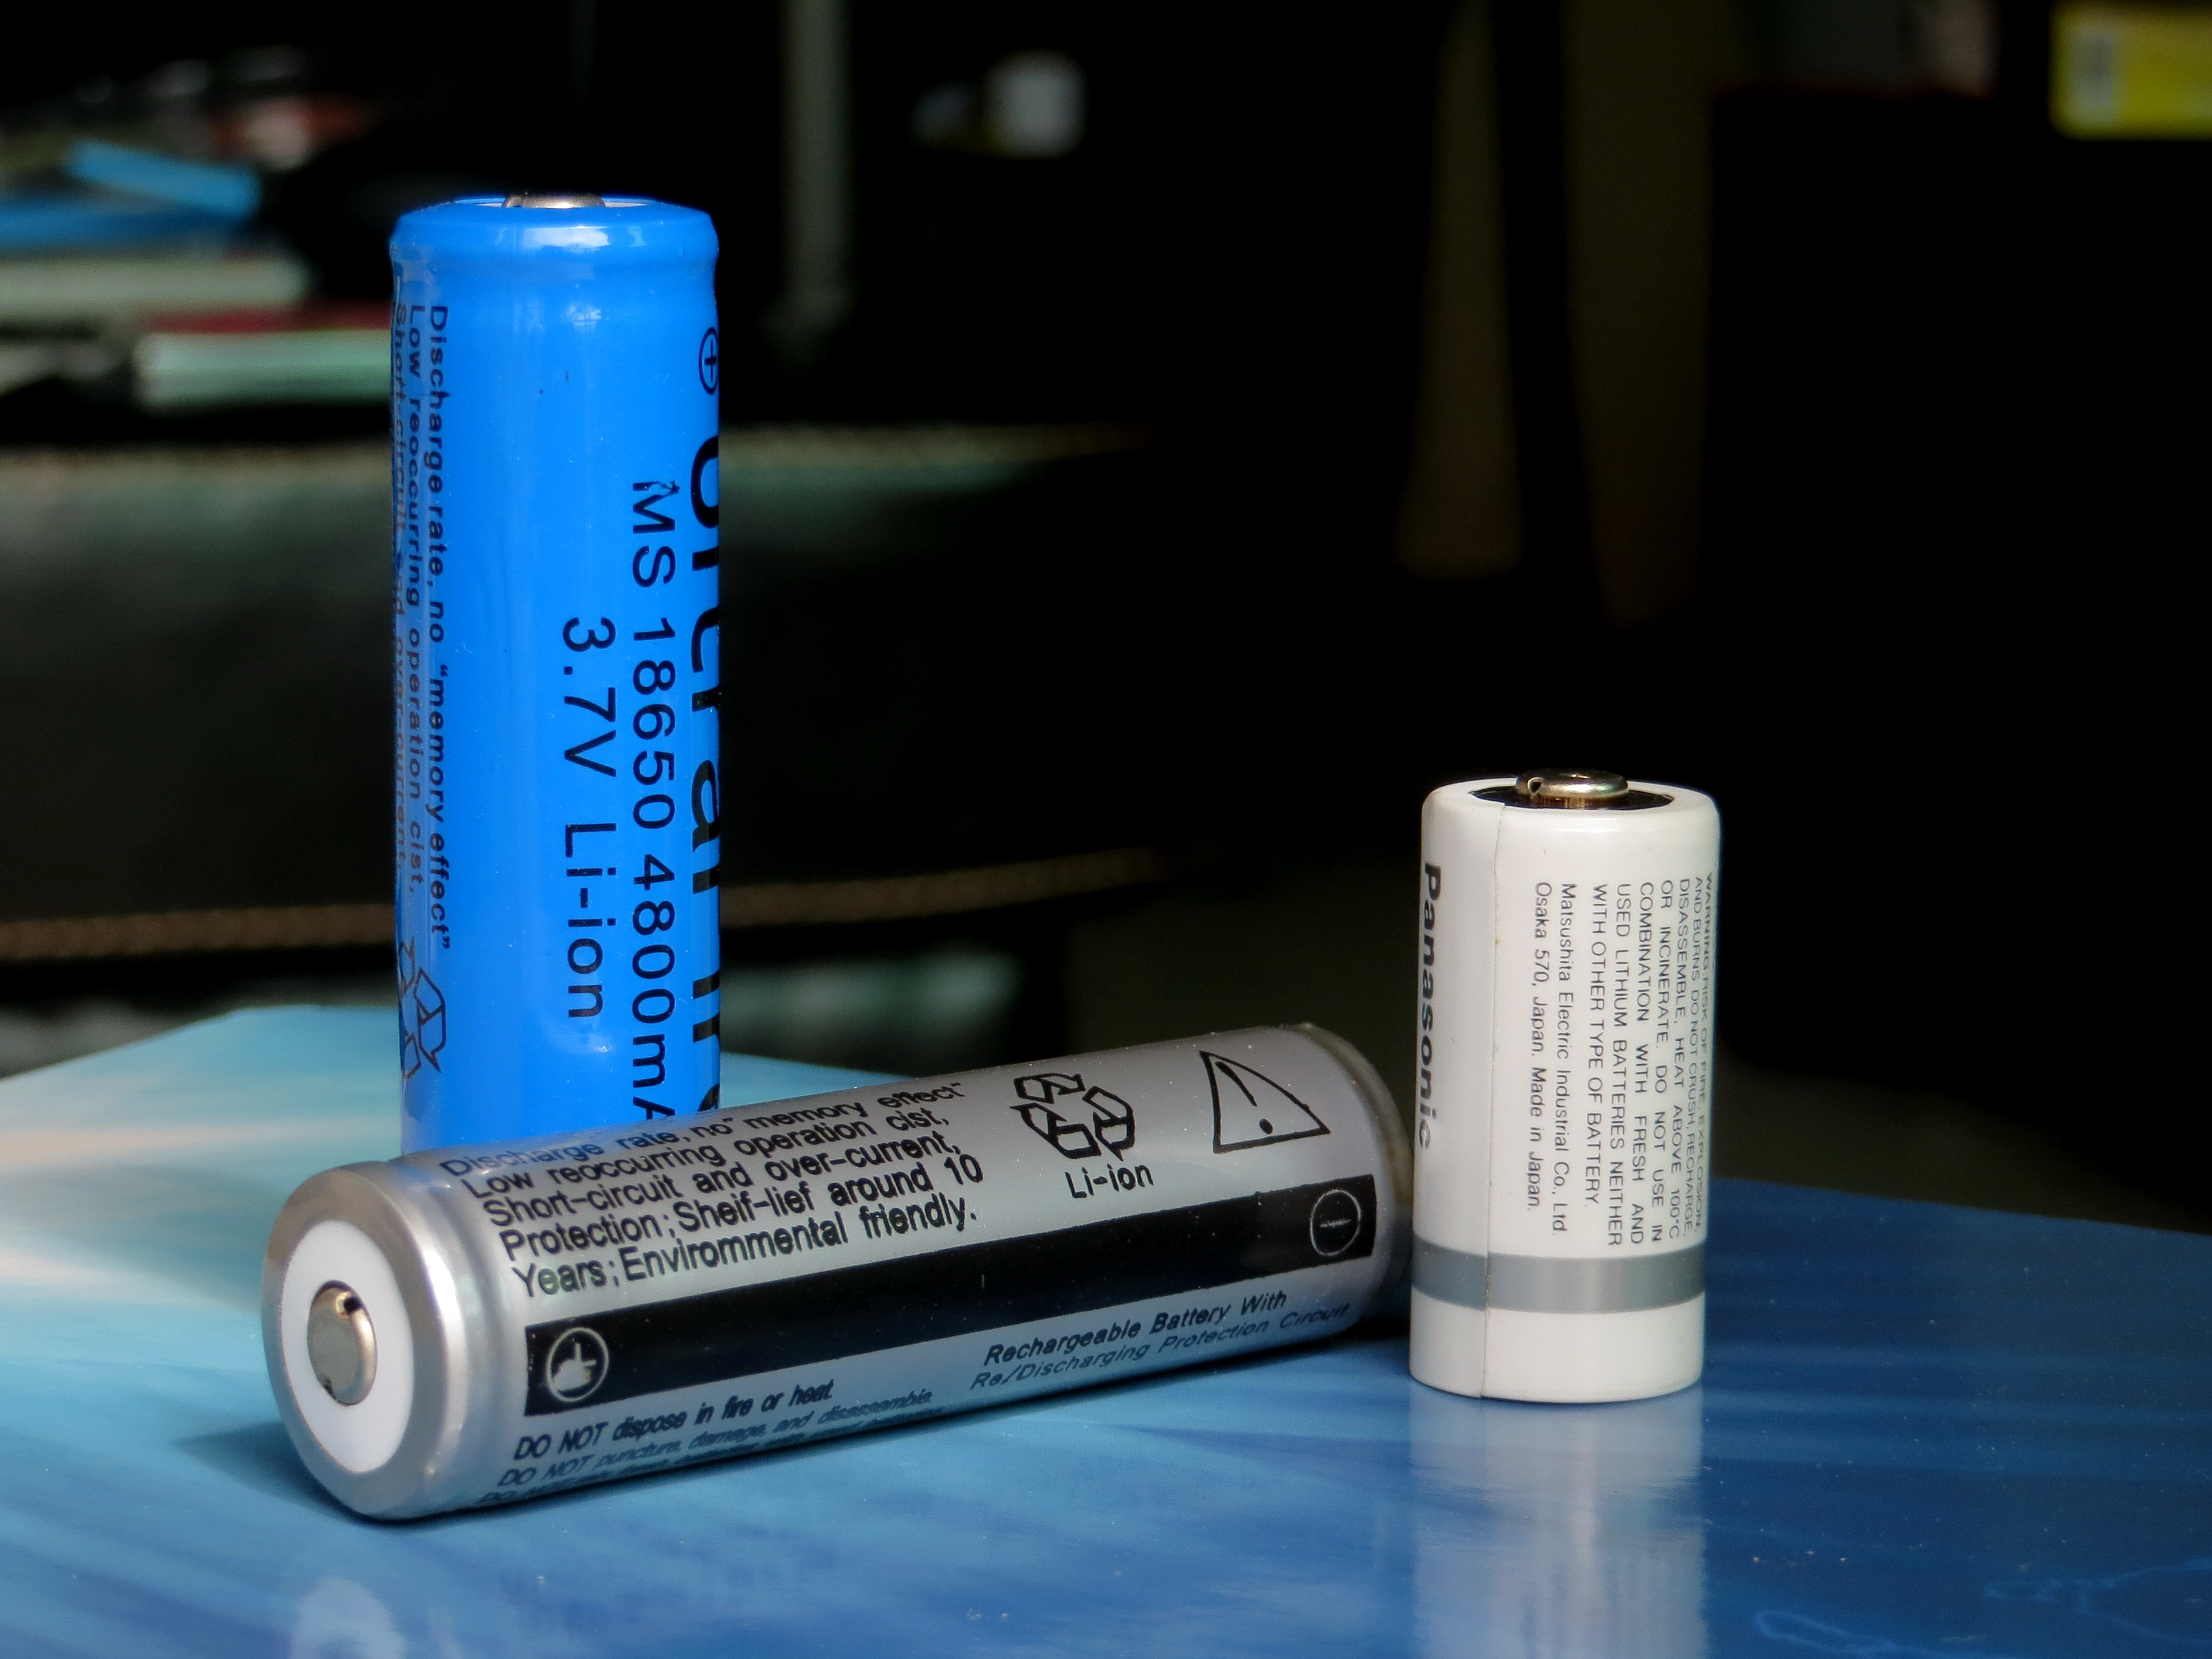
\includegraphics[scale=0.1]{imagenes/Li-ion.jpg}
   \caption{Baterías Li-ion \cite{mk2010_english_2012} }
   \label{fig:liion}
\end{figure}


\subsection{Algoritmos de carga para baterías Li-ion}
\label{sec:alg_lion}
Para la carga de las baterías Li-ion, el método más conocido es el de corriente constante-voltaje constante (CC/VC), esto 
debido a la simplicidad y fácil implementación. Durante la primera etapa de este algoritmo, se aplica una corriente constante
a la batería, hasta que el voltaje de esta alcance un valor preestablecido ($V_{preset}$), usualmente 4.2 voltios, luego se aplica 
un voltaje constante $V_{preset}$ a la batería de forma que la corriente aplicada va reduciendo su valor hasta alcanzar un valor
preestablecido, usualmente 0.1C, donde C es la capacidad de carga de la batería (en mAh), momento en el cual se considera finalizada la 
carga de la bateria \cite{shen_charging_2012}.

\begin{figure}[H]
   \centering
   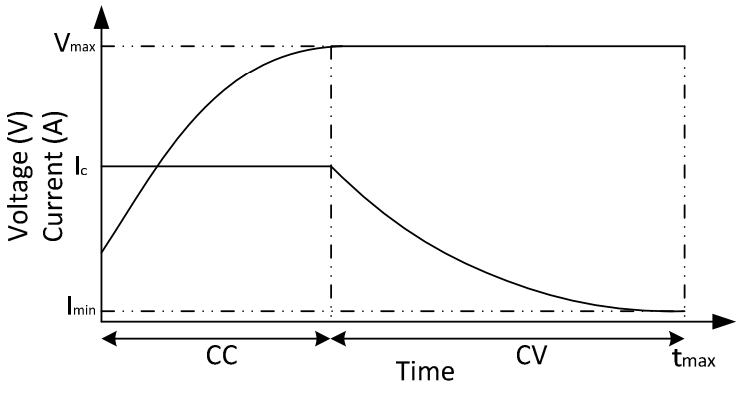
\includegraphics[scale=.6]{imagenes/perfil de carga CC-CV.png }
   \caption{Perfil de carga para el algoritmo CC/VC \cite{shen_charging_2012} }
   \label{fig:cccv}
\end{figure}


Otro algoritmo para la carga de baterías Li-Ion es el denominado \textit{Multistage current charging algorithm} (MSCC). En este
algoritmo se propone el uso de distintos valores de corriente preestablecidos  a los cuales se cargará la batería,
usualmente el cambio entre cada nivel de corriente es establecido cuando el voltaje de carga alcanza un valor determinado
(usualmente 4.2V) \cite{shen_charging_2012}. 


\begin{figure}[H]
   \centering
   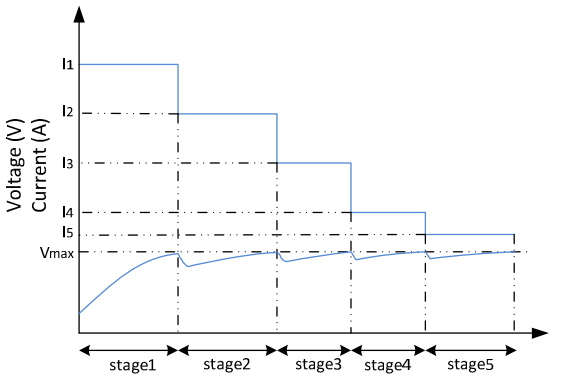
\includegraphics[scale=.75]{imagenes/perfil de carga multietapa.png}
   \caption{Perfil de carga para el algoritmo MSCC \cite{shen_charging_2012}}
   \label{fig:MSCC}
\end{figure}


\section{Baterías de Níquel metalhidruro (NiMH)}

La química de las baterías NiMH cuentan con una tecnología consolidada y ampliamente adoptada. Este tipo de baterías
tienen un menor costo comparado con las baterías basadas en litio. Los métodos de carga para este tipo de baterías son
flexibles ofreciendo corrientes de carga superiores a 1C, o una carga con corrientes bajas, lo cual reduce la demanda
de potencia hacia el sistema de alimentación, y simplificando el circuito de carga. Este tipo de baterías ofrecen altas
corrientes de descarga debido a su baja impedancia interna. Una desventaja de estas baterías es su voltaje nominal 
el cual es de 1.2V, por lo que en aplicaciones típicas es requerido el uso de 3 o 4 celdas en serie
 \cite{texas_instrumens_multi-chemistry_2022}. La densidad energética de este tipo de baterías se encuentra en el 
 rango de 40-60 Wh/Kg \cite{zhan_characteristics_1999}. En la figura \ref{fig:NiMH} se muestran dos baterías NiMH
 en formato AA.

\begin{figure} [H]
   \centering
   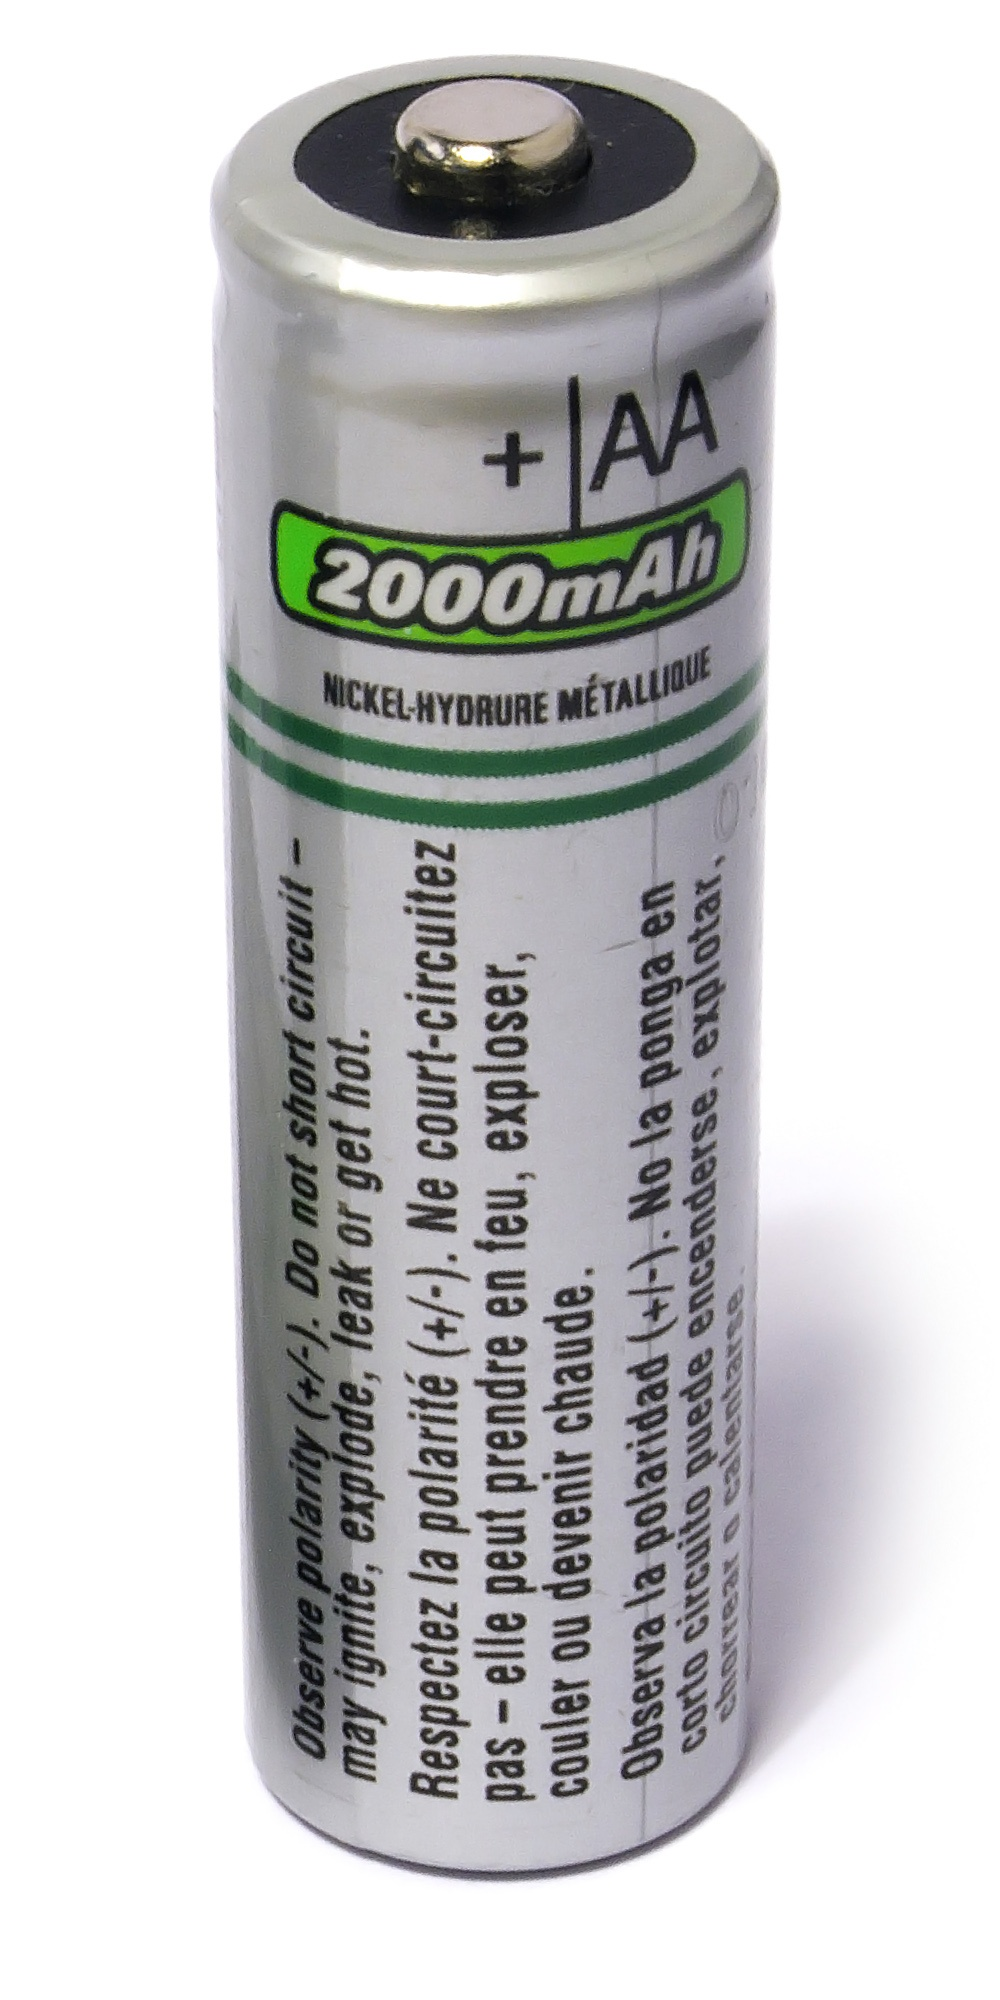
\includegraphics[scale=.1]{imagenes/NiMH.jpg}
   \caption{Batería NiMH \cite{multicherry_english_2020}}
   \label{fig:NiMH}
\end{figure}


\subsection{Algoritmos de carga para baterías NiMH}
\label{sec:alg_nimh}
El algoritmo de cambio de voltaje negativo (\textit{negative delta voltage method}) es un método de carga empleado
en las baterías NiMH que consiste en aplicar una corriente de carga constante a la batería, mientras se monitorea 
el voltaje de la misma. Para determinar cuando la batería se encuentra totalmente cargada se usa la detección de una 
caída de voltaje en la misma. Sin embargo, este método no es el más recomendado, puesto que la reacción química que se 
presenta al momento de la carga de batería es exotérmico, por lo que al momento de presentar esta caída de voltaje se 
puede presentar un aumento excesivo en la temperatura. Otra característica que hace difícil la implementación de este 
algoritmo, es el hecho de que algunos tipos de baterías NiMH no presentan una caída significativa de voltaje al momento
de alcanzar su capacidad máxima de carga \cite{nicolai_nickel-cadmium_1995}.

Un segundo método de carga consiste en aplicar una corriente de carga constante y 
detectar el punto de inflexión (punto en el que ya no existe cambio
en el voltaje de la batería) en la curva de tensión para finalizar el proceso de carga.
Esto ayuda a prevenir un sobrecalentamiento
excesivo de la batería, lo que a su vez contribuye significativamente a prolongar su vida útil. 
Para la detección del punto de inflexión es necesaria la primera derivada del voltaje de la batería con respecto 
al tiempo, en la práctica esta es aproximada mediante la medición en tiempo real \cite{nicolai_nickel-cadmium_1995}.

Adicionalmente es posible emplear un método de carga denominado \textit{trickle
charge} o en español, carga por goteo. Este método consiste en aplicar una 
corriente de carga constante de un valor muy bajo, usualmente 0.1C, hasta que
el voltaje de la batería alcance un valor preestablecido, típicamente 1.4V, 
momento en el cual se considera que la batería se encuentra totalmente cargada
\cite{microchip_trickle}.
\section{Convertidores conmutados}

En el campo de la electrónica de potencia, el principal elemento que es esencial es el convertidor conmutado, el cual
en general consta de un puerto de potencia de entrada, un puerto de potencia de salida, asi como una señal de control,
un modelo de convertidor conmutado se puede observar en la figura \ref{fig:switching}. La potencia de entrada es procesada
con base en la señal de control del convertidor, produciendo una potencia de salida. Un tipo de convertidor comúnmente utilizado
es el convertidor DC-DC, en el cual un voltaje constante de entrada es convertido a un voltaje constante de salida que tiene 
una magnitud menor o mayor, y en algunos casos con polaridad opuesta. Adicionalmente la entrada del convertidor puede o no estar  aislada eléctricamente de la salida. Los convertidores conmutados son
ampliamente usados debido a su alta eficiencia, puesto que, teóricamente tienen una eficiencia del 
100\% a diferencia de los reguladores lineales \cite{erickson_fundamentals_2020}.

\begin{figure}[H]
   \centering
   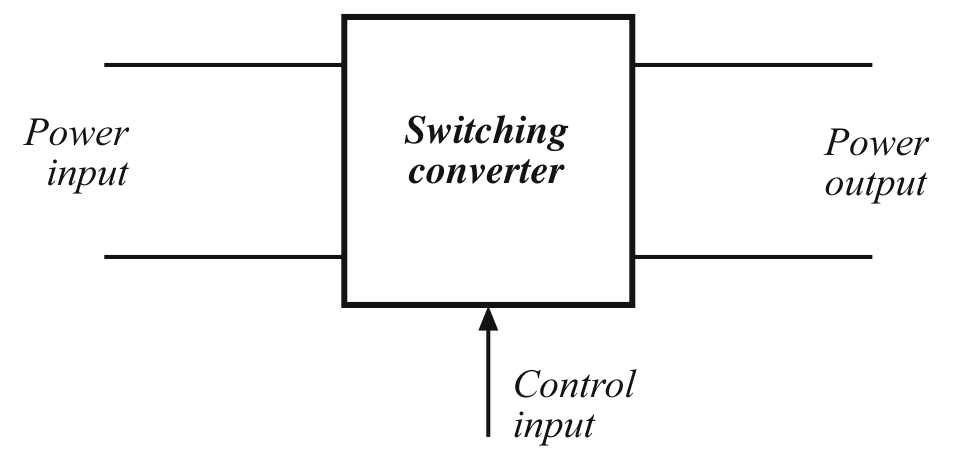
\includegraphics[scale=.4]{imagenes/switching converter.png}
   \caption{Modelo general de un convertidor conmutado \cite{erickson_fundamentals_2020}}
   \label{fig:switching}
\end{figure}

Otra parte esencial para un convertidor conmutado es el controlador,  esto ya que siempre es requerida
un voltaje de salida que se encuentre bien regulado, aun si existen variaciones en el voltaje de entrada
o en la corriente requerida por la carga \cite{erickson_fundamentals_2020}. En la figura \ref{fig:controlador} se 
presenta la topología general para un convertidor conmutado al incluir el controlador. 

\begin{figure}[H]
    \centering
    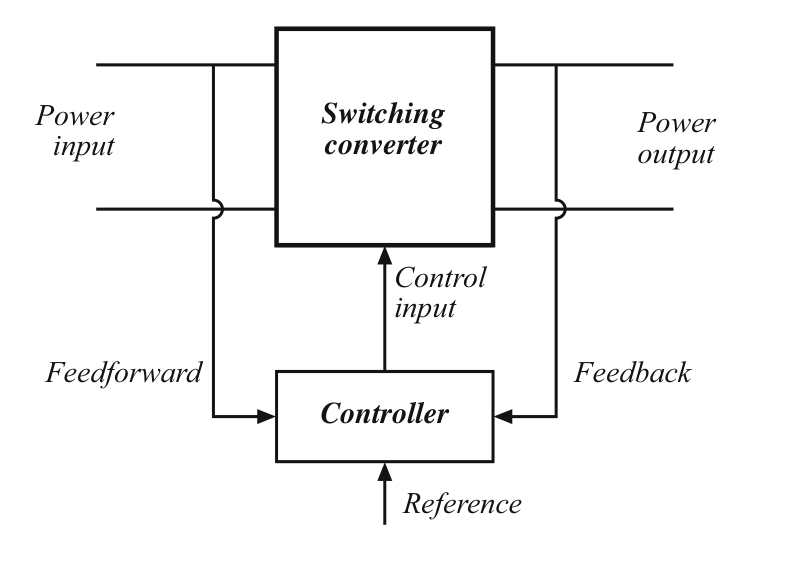
\includegraphics[scale=0.4]{imagenes/topologia.png}
    \caption{Topología general de un convertidor conmutado junto con su controlador \cite{erickson_fundamentals_2020}}
    \label{fig:controlador}
\end{figure}

Los convertidores conmutados DC-DC operan bajo dos principios el balance voltios-segundo en el inductor y el balance en la carga del capacitor, los cuales son explicados a continuación \cite{erickson_fundamentals_2020}.


\subsection{Balance voltios-segundo en el inductor}

 Este principio expresa que el cambio neto en la corriente del inductor
durante un periodo de conmutación debe ser igual a 0, debido a que en un convertidor conmutado
la corriente promedio de un inductor no debe de cambiar. Dado que la relación voltaje-corriente en un  inductor está dada por
\begin{equation}
    v_L = L \odv[order=1]{i_L}{t}
    \label{eq:VIinductor}
\end{equation}

donde $i_L$ es la corriente en el inductor, $v_L$ es el voltaje en el inductor
y $L$ la inductancia, al integrar \ref{eq:VIinductor} durante un periodo de conmutación
se tiene 
\begin{equation}
i_L\left(T_s\right)-i_L(0)=\frac{1}{L} \int_0^{T_s} v_L(t) d t
\label{eq:integralInductor}
\end{equation}

donde $T_s$ es el periodo de conmutación. En la ecuación \ref{eq:integralInductor}, el lado
derecho de la igualdad representa el cambio neto durante un periodo de conmutación, el cual 
debe ser igual a 0, teniendo como resultado

\begin{equation}
    \int_0^{T_s} v_L(t) d t = 0
\end{equation}

este resultado es importante para el análisis de convertidores DC-DC conmutados \cite{erickson_fundamentals_2020}.

\subsection{Balance en la carga del capacitor}

Este principio expresa que el cambio neto de la corriente en el capacitor durante un periodo 
de conmutación es igual a 0. Por argumentos similares a los dados en la sección anterior se 
llega a la ecuación mostrada en \ref{eq:balanceCarga} \cite{erickson_fundamentals_2020}.

\begin{equation}
    \int_0^{T_s} i_C(t) d t = 0
    \label{eq:balanceCarga}
\end{equation}

\subsection{Convertidor reductor (\textit{buck converter})}

El convertidor reductor, como su nombre lo indica, lleva a cabo la función de disminuir
 el voltaje de entrada ($V_g$, en la figura \ref{fig:buck}). Mediante el uso del principio del
balance voltios-segundo en el inductor, el balance en la carga del capacitor, y
 adicionalmente empleando la aproximación de rizado pequeño (aproximación en la cual todos los 
voltajes y corrientes en los elementos de un circuito se consideran constantes  \cite{erickson_fundamentals_2020}),
 se obtiene que la relación entre el voltaje de entrada y el de salida está dado por 
 \begin{equation}
    V=DV_g  
    \label{eq:salida_buck}
 \end{equation}
donde $D$ es el ciclo de trabajo, que es la fracción de tiempo en la que el
interruptor se encuentra en la posición 1 (ver figura \ref{fig:buck}) con
respecto al periodo de conmutación, mientras que $V$ es el voltaje 
a la salida del convertidor ($v(t)$, en la figura \ref{fig:buck})
 \cite{erickson_fundamentals_2020}. 



\begin{figure}[H]
    \centering
    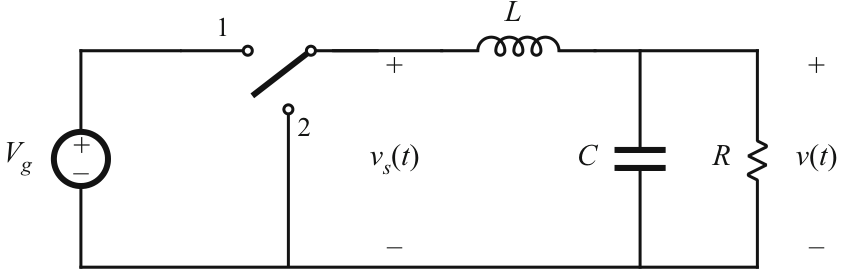
\includegraphics[scale=0.5]{imagenes/buckIdeal.png}
    \caption{Convertidor reductor con elementos ideales \cite{erickson_fundamentals_2020}}
    \label{fig:buck}
\end{figure}

Debido a que para la deducción de la relación entre voltaje de salida y 
entrada del convertidor (ecuación \ref{eq:salida_buck}) fue empleada la
aproximación de rizado pequeño, no se refleja el ruido de conmutación 
a la salida del circuito. En \cite{erickson_fundamentals_2020} se 
realiza el análisis para determinar las amplitudes, para el rizado tanto de 
la corriente del inductor como del voltaje en el capacitor (ecuaciones 
\ref{eq:ripple_L} y \ref{eq:ripple_C} respectivamente)
\begin{equation}
    \Delta I = \frac{V_g-V}{2L}DT_s
    \label{eq:ripple_L}
\end{equation}

\begin{equation}
    \Delta C = \frac{\Delta I T_s}{8C}
    \label{eq:ripple_C}
\end{equation}

En las figuras \ref{fig:ripple_L} y \ref{fig:ripple_C} se puede observar la forma de onda del voltaje
en el capacitor y la corriente en el inductor del convertidor reductor.

\begin{figure}[H]
    \centering
    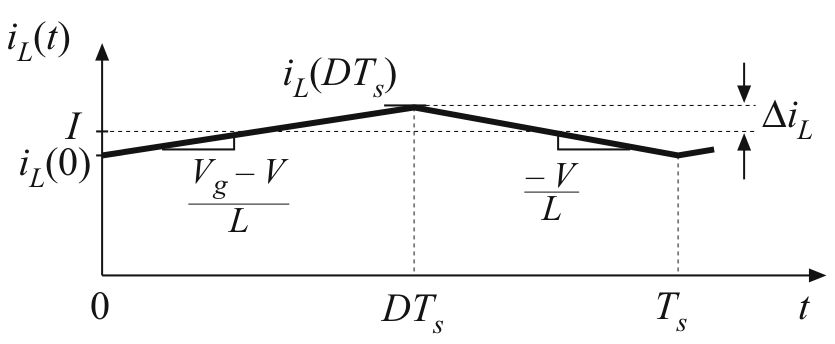
\includegraphics[scale=.5]{imagenes/buck_ripple_L.png}
    \caption{Forma de onda de la corriente en el inductor \cite{erickson_fundamentals_2020}}
    \label{fig:ripple_L}
\end{figure}

\begin{figure} [H]
    \centering
    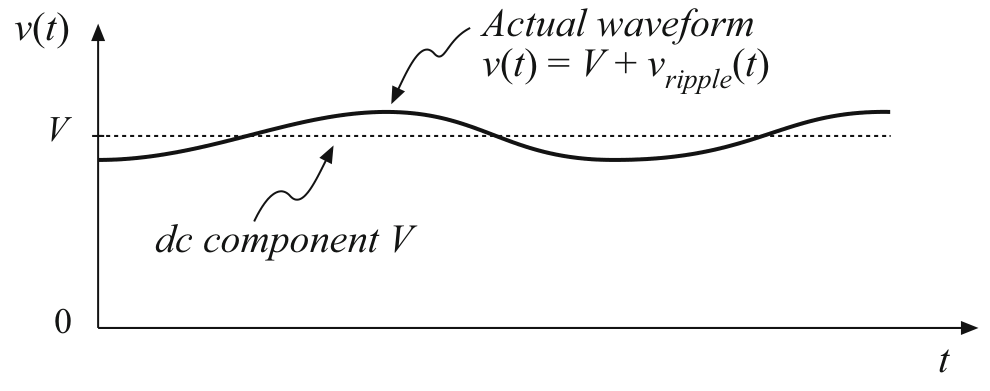
\includegraphics[scale=.4]{imagenes/buck_ripple.png}
    \caption{Forma de onda del voltaje en el capacitor \cite{erickson_fundamentals_2020}}
    \label{fig:ripple_C}
\end{figure}

\subsubsection{LM2596}

 El LM2596 es un IC el cual permite el diseño de un convertidor reductor que opera a una 
 frecuencia de $150\text{KHz}$ con conmutador integrado
por lo que únicamente es necesario añadir un inductor, diodo y capacitor de 
 forma externa para tener un convertidor reductor. 
 
 Este viene en versiones con voltajes de 
 salida fijos y también con una versión ajustable.  Para la versión ajustable la tensión de
 referencia es de 1.23 V de forma típica, este voltaje de referencia es el que busca igualar
 el controlador interno en el pin denominado \textit{feedback}. Para establecer el voltaje
 a la salida es necesario añadir 2 resistencias funcionando como divisor de voltaje, 
 de forma que se le permita al IC sensar el voltaje de salida. Para la determinación de los
valores de resistencias es utilizada la ecuación \ref{eq:lm2596}. 

 \begin{figure}[H]
    \centering
    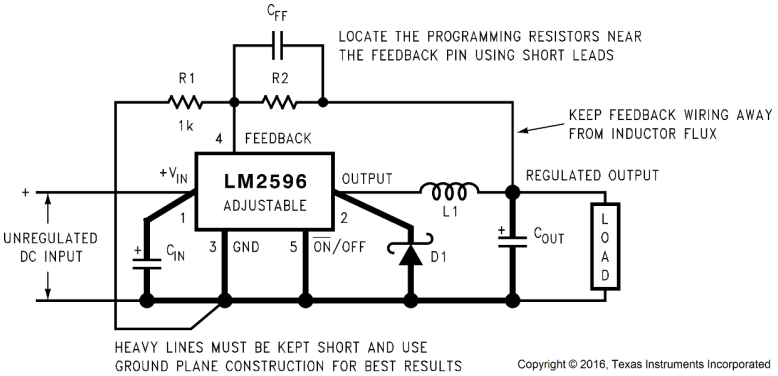
\includegraphics[scale=0.7]{imagenes/LM2596_adj.png}
    \caption{Convertidor reductor utilizando el LM2596 en su versión ajustable \cite{lm2596}}
    \label{fig:lm2596}
 \end{figure}
 
\begin{equation}
    R_2 = R_1(\frac{V_{out}}{V_{ref}} - 1)
    \label{eq:lm2596}
\end{equation}

En donde $R_1$ y $R_2$ son los las resistencias con los mismos nombres mostrados en la
figura \ref{fig:lm2596} mientras que $V_{ref}$ es el voltaje de referencia interno del
IC, y $V_{out}$ es el voltaje de salida deseado. Es posible desactivar el funcionamiento
del LM2596 aplicando un voltaje superior a 2 V, en el pin 
$\overline{\text{ON}}\backslash\text{OFF}$.

\subsection{Multiplicador de voltaje (\textit{Charge pump})}
    \label{sec:charge_pump}
    Un multiplicador de voltaje es un convertidor conmutado que permite (idealmente)
    obtener un voltaje de salida que es múltiplo entero del voltaje de entrada
    (ver ecuación \ref{eq:charge_pump}).
    
    \begin{equation}
        V_{out} = n V_{in}
        \label{eq:charge_pump}
    \end{equation}
    
    Un circuito empleado comúnmente es denominado \textit{
    Dickson charge pump} el cual es mostrado en la figura \ref{fig:dickson_charge}.
    
    \begin{figure}[H]
        \centering
        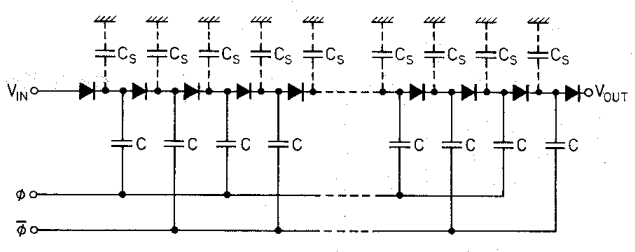
\includegraphics[scale=1]{imagenes/Positive_dickson_charge.png}
        \caption{\textit{ Dickson charge pump} \cite{charge_dikson}}
        \label{fig:dickson_charge}
    \end{figure}

    En \cite{charge_dikson} se realiza el análisis del circuito mostrado
    en la figura \ref{fig:dickson_charge}, con
    el cual se obtiene que la relación entre voltaje de entrada y salida está dada
    por la ecuación \ref{eq:dickson_charge}.

    \begin{equation}
        V_{out} = V_{in} + N \left (  \frac{C}{C+C_s}V_\Phi - V_D - 
        \frac{I_{out}}{(C+C_s)f} \right ) - V_D
        \label{eq:dickson_charge}
    \end{equation}

    En donde $N$ es el número de etapas en el convertidor, $C$ es la capacitancia
    entre cada etapa y el nodo $\Phi$ o $\bar{\Phi}$, $f$ es la frecuencia de 
    operación del multiplicador de voltaje, $V{\Phi}$ es la amplitud
    de la señal en los nodos $\Phi$ y $\bar{\Phi}$, $C_s$ son capacitancias parásitas,
    $I_{out}$ es la corriente de salida del
    convertidor y $V_D$ es la caída de voltaje en el diodo.

    Este mismo convertidor puede ser empleado para obtener un voltaje de salida
    menor al de entrada (es decir voltajes negativos), para ello es necesario
    realizar un intercambio entre la carga del circuito y el voltaje de entrada,
    Por lo que en la ecuación \ref{eq:dickson_charge} $V_{in}$ y $V_{out}$
    son intercambiados \cite{mohammad_switched_2010}. En la figura 
    \ref{fig:dickson_charge_bid} se muestra el intercambio entre carga y 
    voltaje de entrada en el \textit{Dickson charge pump}.
    
    \begin{figure}[H]
        \centering
        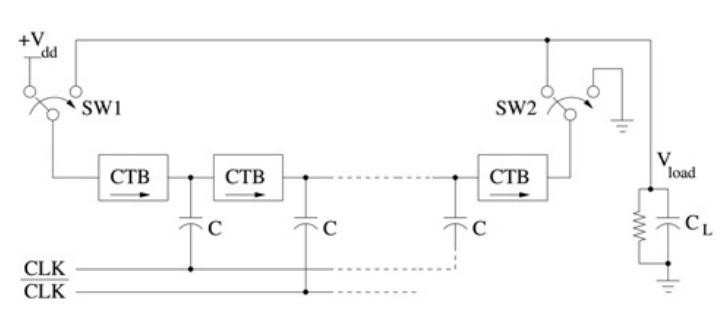
\includegraphics[scale=0.75]{imagenes/positive_negative_charge_pump.png}
        \caption{intercambio entre carga y voltaje de entrada en el
                 \textit{Dickson charge pump} (CTB, \textit{charge transfer
                 block} en la figura \ref{fig:dickson_charge} son implementados
                 con diodos) \cite{mohammad_switched_2010}}
        \label{fig:dickson_charge_bid}
    \end{figure}

    Al intercambiar el voltaje de entrada y salida de la ecuación \ref{eq:dickson_charge},
    y aplicando $0$V en la entrada (que es el caso mostrado en la figura 
    \ref{fig:dickson_charge_bid}, cuando SW1 y SW2 se encuentran cerrados 
    con el contacto de la derecha) se tiene que la relación entre voltaje de entrada
    y salida está dada por la ecuación \ref{eq:dickson_charge_neg}.

    \begin{equation}
        V_{out} = - N \left (  \frac{C}{C+C_s}V_\Phi - V_D - 
        \frac{I_{out}}{(C+C_s)f} \right ) + V_D
        \label{eq:dickson_charge_neg}
    \end{equation}


\section{Multiplexores de potencia}

Un multiplexor de potencia, es un conjunto de conmutadores electrónicos que son utilizados
para seleccionar entre dos o más entradas de potencia, hacia una única salida. El uso de 
multiplexores de potencia le brinda la flexibilidad a un sistema de poder seleccionar
entre diferentes tipos de entradas de potencia \cite{triano_basics_2020}. En la figura 
\ref{fig:powerMux} se muestra el diagrama de bloques de un multiplexor de potencia.


\begin{figure}[H]
    \centering
    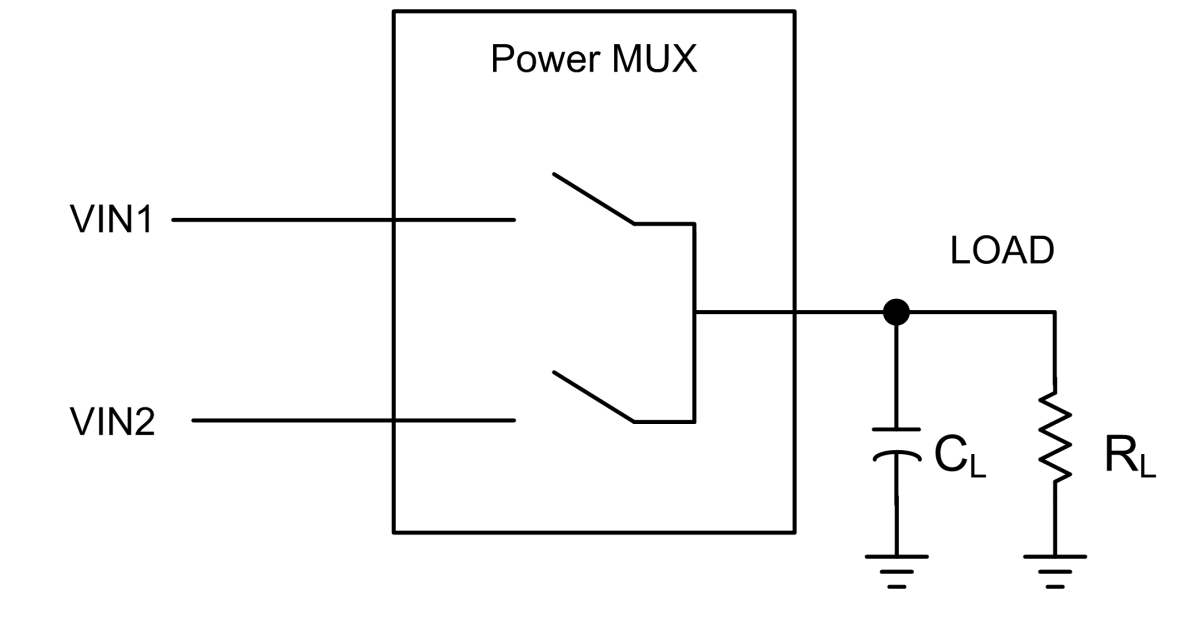
\includegraphics[scale=.35]{imagenes/powerMux.png}
    \caption{Diagrama de bloques de un multiplexor de potencia \cite{triano_basics_2020}}
    \label{fig:powerMux}
\end{figure}


En el caso de que no exista preferencia para alguna de las alimentaciones de entrada, o inclusive
si siempre se prefiere el uso del voltaje de entrada más alto, el requerimiento mínimo para un multiplexor
de potencia es el bloqueo de corriente inversa. Este requerimiento puede ser cumplido mediante el uso de 
diodos o circuitos integrados que se comporten como diodos \cite{triano_basics_2020}.  Como se muestra en la figura \ref{fig:muxDiode}.

\begin{figure}[H]
    \centering
    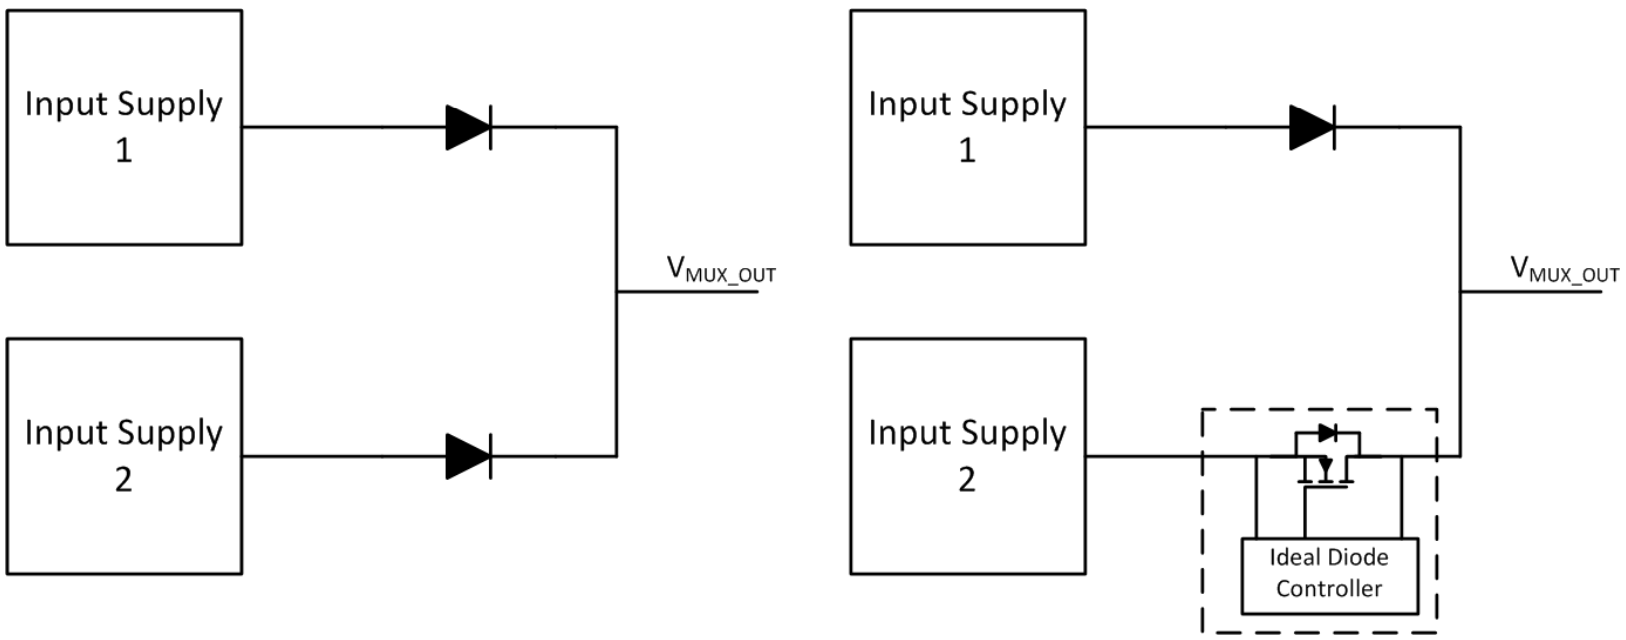
\includegraphics[scale=.3]{imagenes/minimumMux.png}
    \caption{Sistema mínimo para un multiplexor de potencia \cite{triano_basics_2020}}
    \label{fig:muxDiode}
\end{figure}

En el caso de que exista alguna prioridad para los voltajes de entrada, es necesario agregar conmutadores,
por ejemplo un transistor MOSFET, para tener un control total sobre la ruta que será habilitada. Al igual que
en el caso sin prioridad, el bloqueo ante corrientes inversas debe seguir presente \cite{triano_basics_2020}. En la figura \ref{fig:priorityMux} se muestra un ejemplo de multiplexor de potencia con prioridad.

\begin{figure}[H]
    \centering
    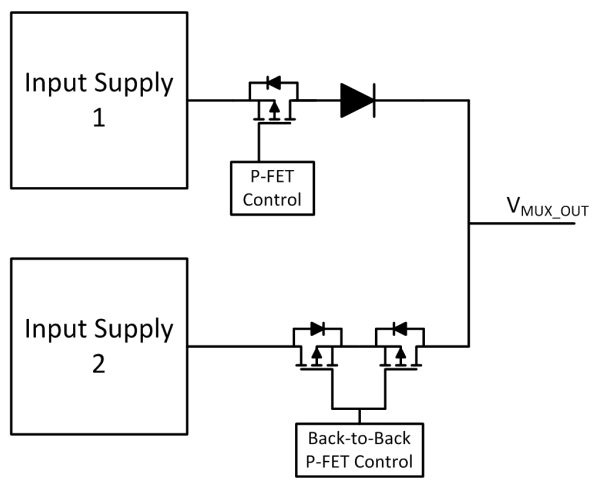
\includegraphics[scale=.4]{imagenes/priorityMUX.png}
    \caption{Multiplexor de potencia con prioridad \cite{triano_basics_2020}}
    \label{fig:priorityMux}
\end{figure}

Para el control de multiplexores de potencia, se tienen dos opciones: manual o automático. Un multiplexor de
potencia manual es aquel en el cual cada fuente de alimentación es seleccionada mediante señales externas. Por el contrario, un multiplexor automático es aquel que no requiere señales externas para el cambio entre 
una fuente de alimentación y otra, en este tipo de control usualmente existe una entrada de potencia que 
tiene la prioridad.

\section{Pololu 3Pi+}

El Pololu 3Pi+ es un robot, programable por el usuario. Este se encuentra basado en el microcontrolador ATmega32U4 AVR
de microchip, el microcontrolador incorporado se encuentra preprogramado con un gestor de arranque que es compatible
 Con la plataforma Arduino. Incluye dos puentes H para el control de los motores así como distintos sensores, como lo 
 son \textit{encoders} de cuadratura, así como una unidad de medición inercial \cite{noauthor_pololu_nodate}. En cuanto 
 al sistema de potencia tiene como principal fuente de energía el uso de cuatro celdas AAA en serie, en donde el 
 terminal negativo se encuentra conectado a GND mientras que el terminal positivo, al pin denominado VBAT (ver figura
 \ref{fig:power}).

 \begin{figure}[H]
    \centering
    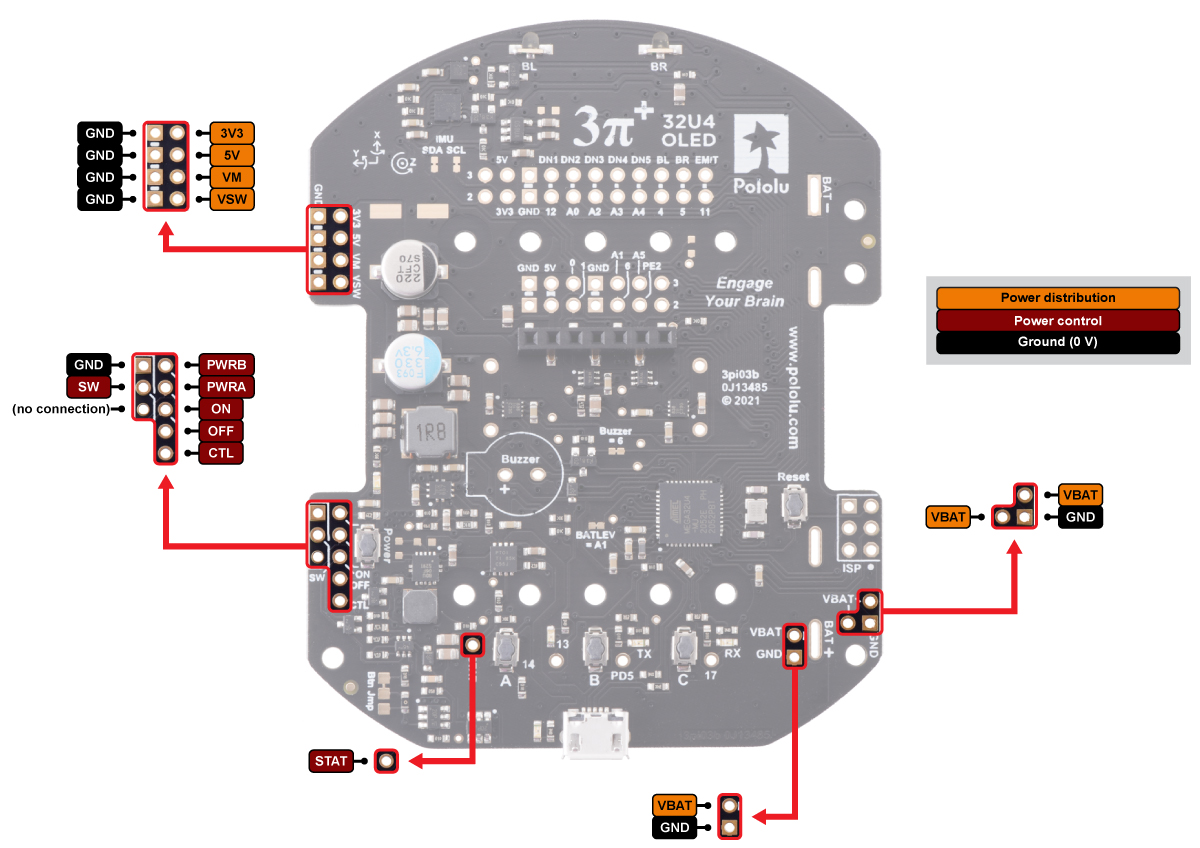
\includegraphics[scale=.2]{imagenes/PololuPower.jpg}
    \caption{Distribución de los pines de potencia el Pi3+ \cite{noauthor_pololu_nodate}}
    \label{fig:power}
 \end{figure}

 Para la alimentación de los motores, el Pi3+ posee un convertidor conmutado, para proveer de 8 voltios a los motores
 de forma que no se presente una caída en la velocidad de los motores debido a la descarga gradual de las baterías,
 adicionalmente, se tiene un segundo regular conmutado que provee 5 voltios, aunque esta no es accesible de forma directa
 para el usuario. También posee un regulador lineal (LDO por sus siglas en inglés). El voltaje de entrada (el cual es 
 utilizado para generar los 8, 5 y 3.3 voltios de la placa) es seleccionado mediante un multiplexor de potencia, más 
 específicamente se emplea el circuito integrado (IC) TPS2113A fabricado por Texas Instruments \cite{noauthor_pololu_nodate}.

\section{Amplificador operacional}

Un amplificador operacional es un amplificador con una alta ganancia,
alta impedancia de entrada y baja impedancia de salida. Posee dos entradas
las cuales son denominadas entrada inversora, entrada no inversora. La salida
del amplificador operacional es la diferencia entre las dos entradas multiplicada
por la ganancia del amplificador operacional \cite{electronic_Boylestad}. En 
la figura \ref{fig:ampOp} se muestra el símbolo de un amplificador operacional.

\begin{figure}[H]
    \centering
    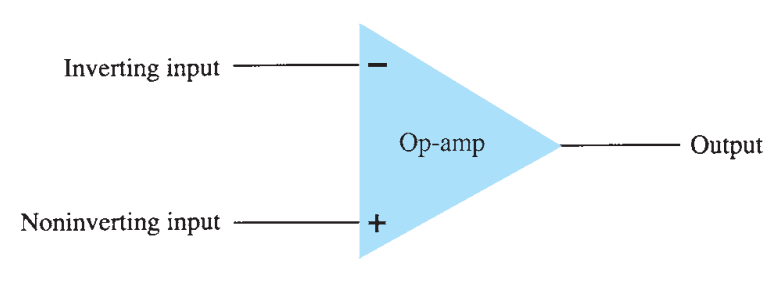
\includegraphics[scale=0.3]{imagenes/ideal_opamp.png}
    \caption{Símbolo de un amplificador operacional \cite{electronic_Boylestad}}
    \label{fig:ampOp}
\end{figure}

La ecuación que describe el comportamiento de un amplificador operacional es la siguiente
\begin{equation}
    V_{out} = A(V^+ - V^-)
    \label{eq:ampOp}
\end{equation}

Una consecuencia de que la ganancia del amplificador operacional sea muy alta, es que
la diferencia entre las entradas inversora y no inversora es muy pequeña, por lo que
se puede considerar que ambas entradas tienen el mismo voltaje. Esta característica
es conocida como "cortocircuito virtual" \cite{electronic_Boylestad}.

 El hecho de tener una 
impedancia de entrada infinita implica que no existe corriente de entrada, por lo que
la corriente que entra por la entrada inversora y no inversora es igual a 0. 

\subsection{Amplificador diferencial}
\label{sec:ampDif}
Un amplificador diferencial es un amplificador operacional que tiene dos entradas
y una salida. La salida de este amplificador es la diferencia entre las dos entradas
multiplicada por la ganancia del amplificador diferencial. En la figura \ref{fig:ampDif}
se muestra el diagrama de un amplificador diferencial \cite{electronic_Boylestad}.

\begin{figure}[H]
    \centering
    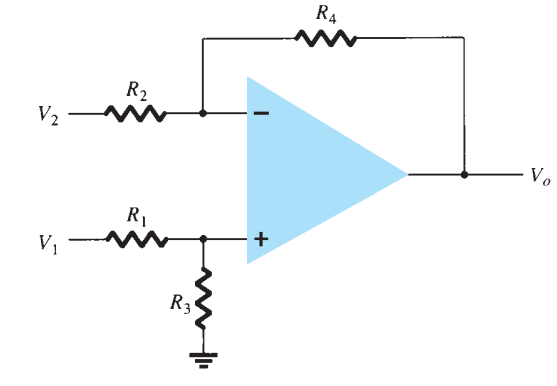
\includegraphics[scale=0.3]{imagenes/ampDif.png}
    \caption{Diagrama de un amplificador diferencial \cite{electronic_Boylestad}}
    \label{fig:ampDif}
\end{figure}

La ecuación que describe el comportamiento de un amplificador diferencial es la siguiente:
\begin{equation}
    V_{out} =  \frac{R_3(R_2+R_4)}{R_2(R_1+R_3)}V_2 - \frac{R_4}{R_2}V_1
    \label{eq:ampDif}
\end{equation}

Si el valor de $R_1$ es igual a $R_2$ y el valor de $R_3$ es igual a $R_4$, la ecuación
\ref{eq:ampDif} se puede simplificar a la ecuación \ref{eq:ampDifSimp}.
\begin{equation}
    V_{out} =  \frac{R_4}{R_2}(V_2 - V_1)
    \label{eq:ampDifSimp}
\end{equation}